% LINGI2251
% Development methods
\documentclass[11pt, a4paper]{article}
\usepackage[utf8]{inputenc}
\usepackage[UKenglish]{babel}
\usepackage{graphicx}				% Use pdf, png, jpg, or eps§ with pdflatex; use eps in DVI mode
\usepackage{xcolor}
\usepackage{listings}
\usepackage{hyperref}
\usepackage{array}
\usepackage{longtable}
\usepackage{multirow}
\usepackage[babel=true]{csquotes}


\usepackage[T1]{fontenc}

\lstset{%
	basicstyle=\ttfamily\footnotesize,
	commentstyle=\color{green!90!black},
	frame=single,
	keywordstyle=\bfseries\color{blue},
	language=Java,
	numberstyle=\color{gray},
	showstringspaces=false,
	tabsize=4,
}


\hypersetup{%
	colorlinks=true,
	linkcolor=blue,
	urlcolor=blue
}


\newcommand{\tbf}[1]{\textbf{#1}}
\newcommand{\tit}[1]{\textit{#1}}

\newcommand{\data}[1]{\textit{#1}}
\newcommand{\state}[1]{\textsf{#1}}

\newcommand{\settextlisting}{\lstset{ basicstyle=\small\ttfamily }}
\newcommand{\setcodelisting}{\lstset{ basicstyle=\footnotesize\ttfamily }}



\def\blurb{\textsc{Université catholique de Louvain\\
  École polytechnique de Louvain\\
  Pôle d'ingénierie informatique}}
\def\clap#1{\hbox to 0pt{\hss #1\hss}}%
\def\ligne#1{%
  \hbox to \hsize{%
    \vbox{\centering #1}}}%
\def\haut#1#2#3{%
  \hbox to \hsize{%
    \rlap{\vtop{\raggedright #1}}%
    \hss
    \clap{\vbox{\vfill\centering #2\vfill}}%
    \hss
    \llap{\vtop{\raggedleft #3}}}}%
\begin{document}

\begin{titlepage}
\thispagestyle{empty}\vbox to 1\vsize{%
  \vss
  \vbox to 1\vsize{%
    \haut{\raisebox{-2mm}{
\includegraphics[width=2.5cm]{logo_epl.jpg}}}{\blurb}{\raisebox{-5mm}{
\includegraphics[scale=0.20]{ingi_logo}}}
    \vfill
    \ligne{\Huge \textbf{\textsc{LINGI2251}}}
     \vspace{5mm}
    \ligne{\huge \textbf{\textsc{Development methods}}}
     \vspace{15mm}
    \ligne{\Large \textbf{\textsc{Assignment 2: The Dinoco GSCS}}}
    \vspace{5mm}
    \ligne{\large{\textsc{April 20, 2015}}}
    \vfill
    \vspace{5mm}
    \ligne{%
         \textsc{Professor\\Charles Pecheur}
      }
      \vspace{10mm}
    }%
    \ligne{%
         \textsc{Michael Heraly\\Thibault Gerondal}
      }
      \vspace{5mm}
  \vss
  }
\end{titlepage}



\newpage


\section{Architectural Design}
\subsection{Hierarchical decomposition}

\begin{center}
\centerline{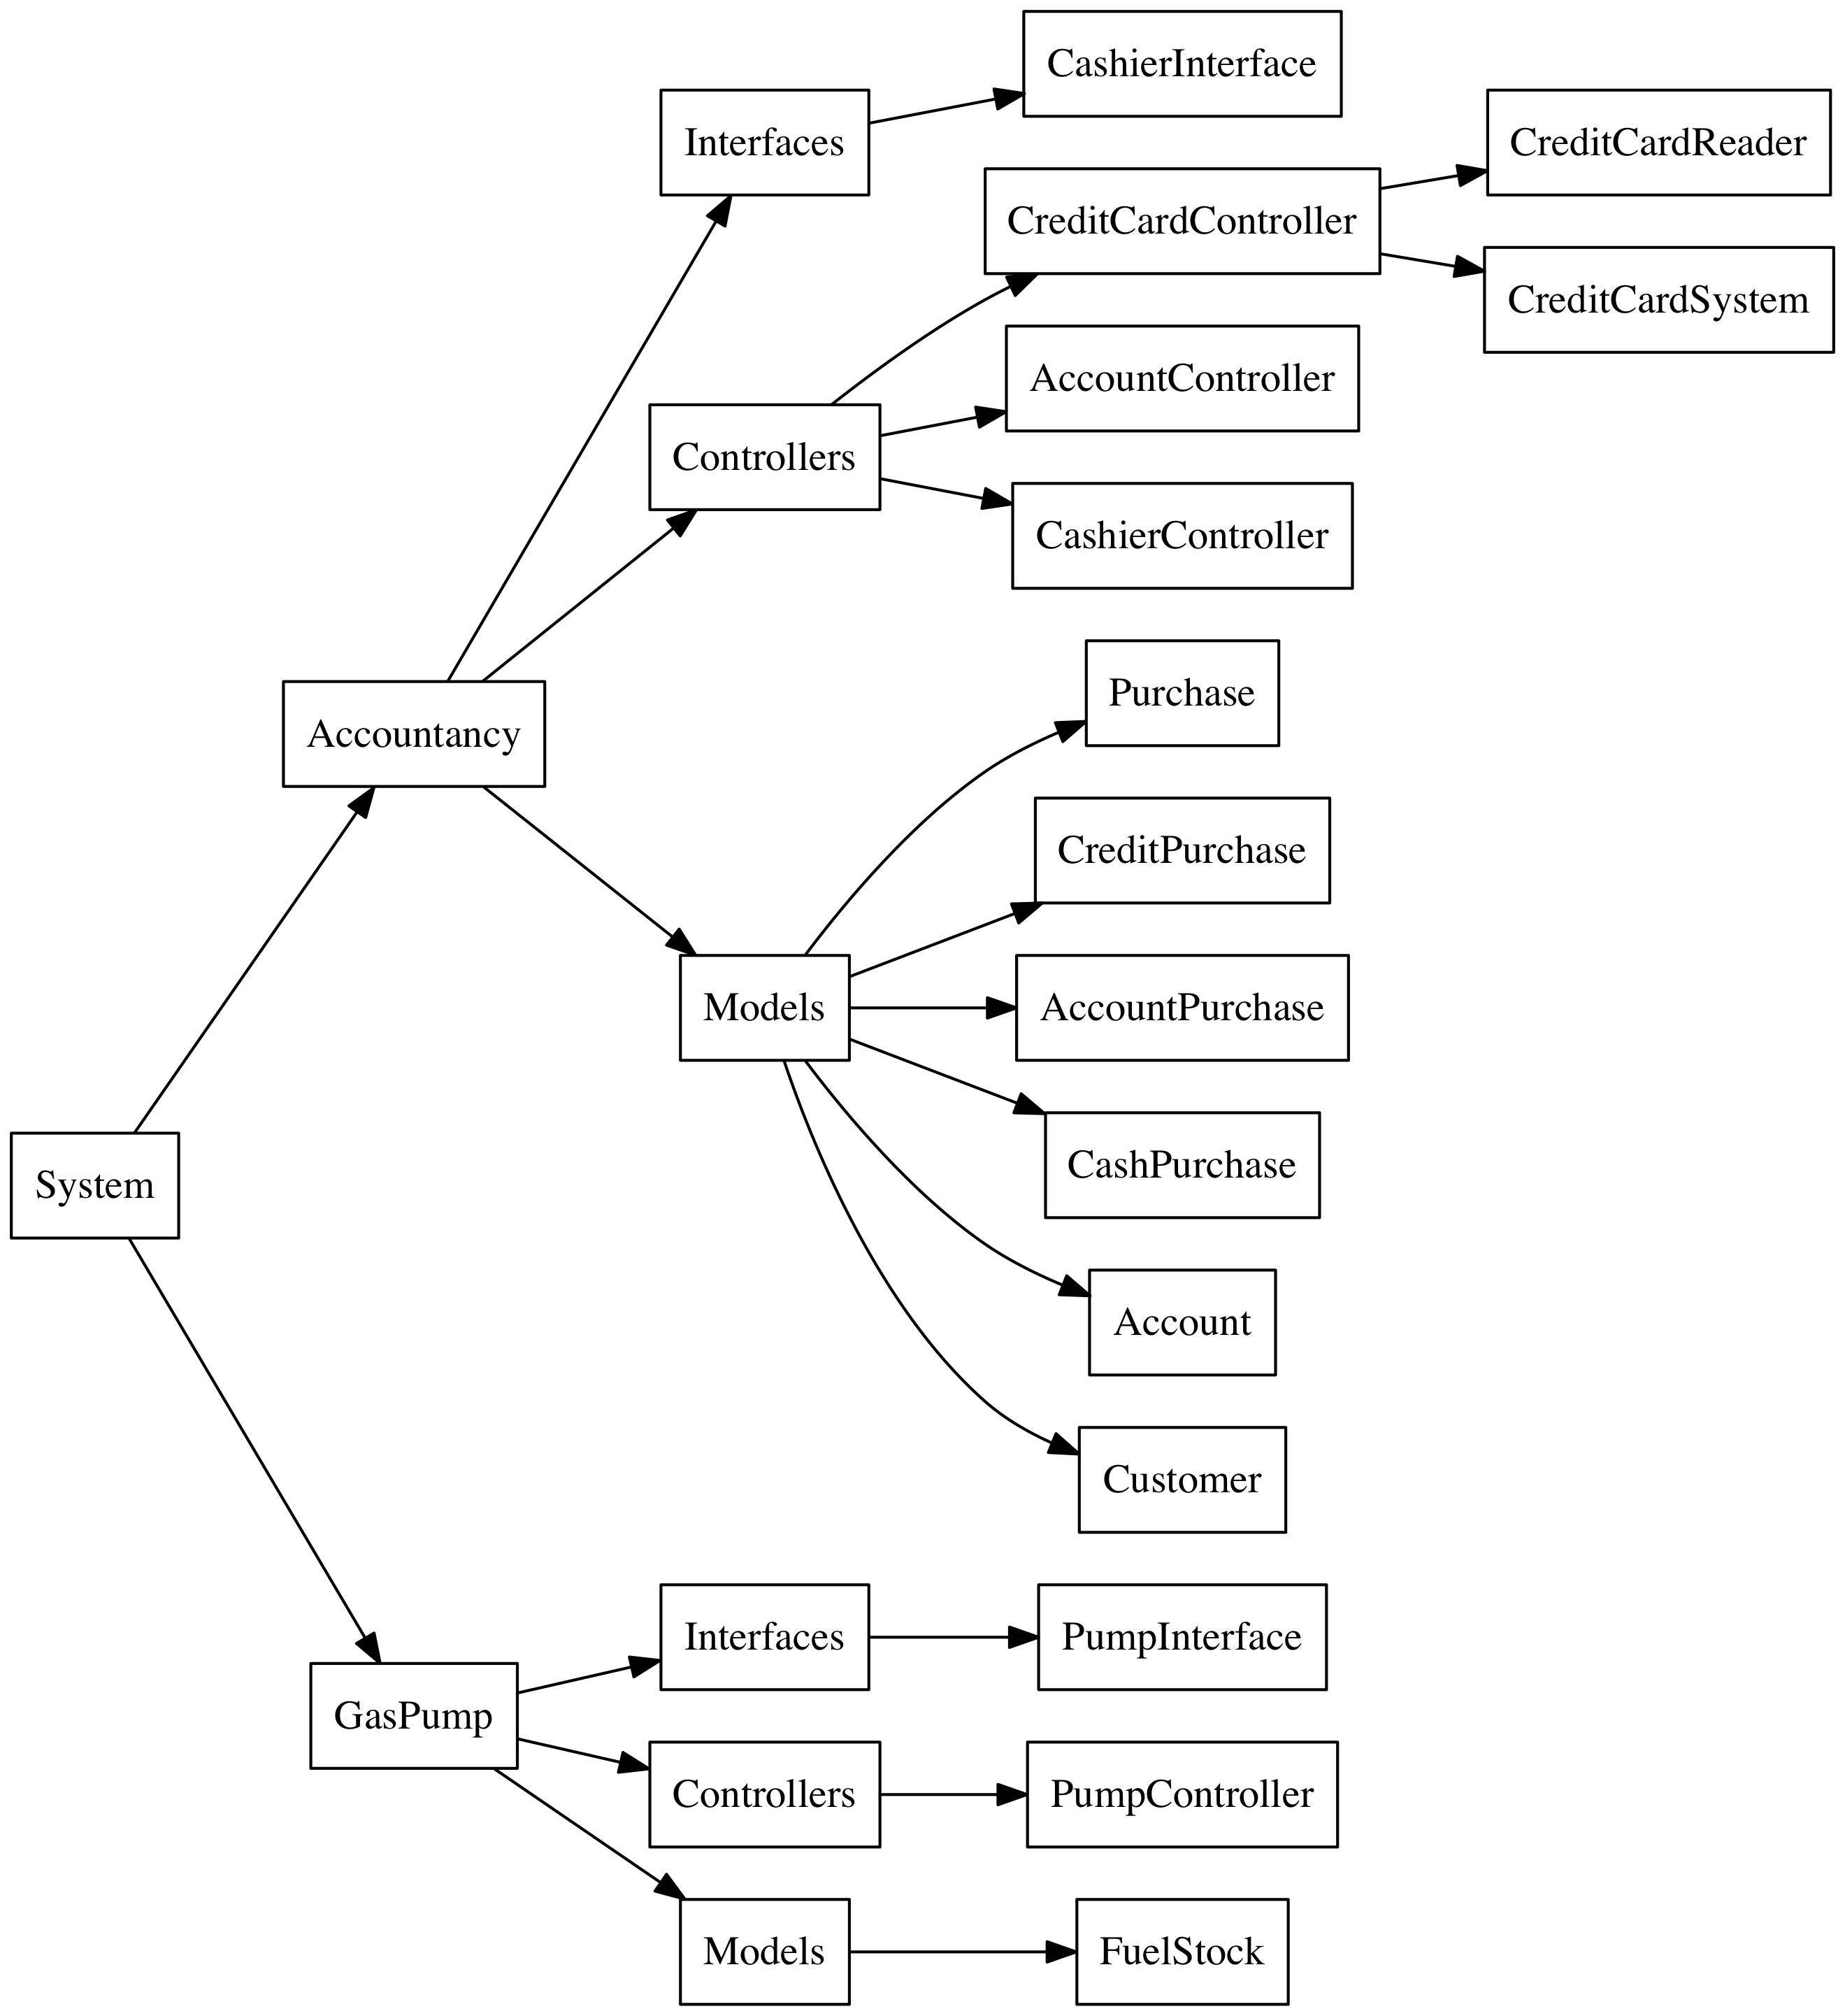
\includegraphics[width=1.3\textwidth]{hierarchical.png}}
\end{center}

\subsection{Roles and interactions}

Our system is composed of two parts : ``Accountancy'' and ``Gas Pump''. The first one is related to accounting. And the second one is about the logistic of the gas pump. This hierarchy allows to easily extend the activities of \textbf{Dinoco GSCS}.\\


In each of these two sections, we defined three main components : ``Interfaces'', ``Controllers'', ``Storages''. \\

\settextlisting
Here are the descriptions of the system components :
\begin{description}
\item[CashierInterface] is responsible for displaying the graphical user interface to the cashier.
\item[AccountController] is responsible for the access to accounts informations (relation to \lstinline|AccountancyStorage|).
\item[CashierController] is responsible for the interactions between the \lstinline|CashierInterface| and the \lstinline|AccountController| (e.g. open a monthly bill, pay a monthly bill, etc.). It also permits the cashier to check the fuel stock from the \lstinline|PumpController| (which will retrieve the information from the \lstinline|FuelStorage|).
\item[DevicesController] is responsible for the interactions between the \lstinline|CreditCardReader| and the \lstinline|CreditCardSystem|.
\item[AccountancyStorage] is responsible for storing the accounts informations.
\item[CreditCardReader] is responsible for reading credit card number (wrapping the existing API for the device).
\item[CreditCardSystem] is responsible for requesting payment (wrapping the existing system API).
\item[PumpInterface] is responsible for displaying informations to the customer.
\item[PumpController] is responsible for the interactions between the \lstinline|PumpInterface| and the Dinoco GSCS.
\item[FuelStorage] is responsible for storing the fuel informations.
\end{description}

\section{Detailed design}
\subsection*{Class diagram}

\begin{center}
\centerline{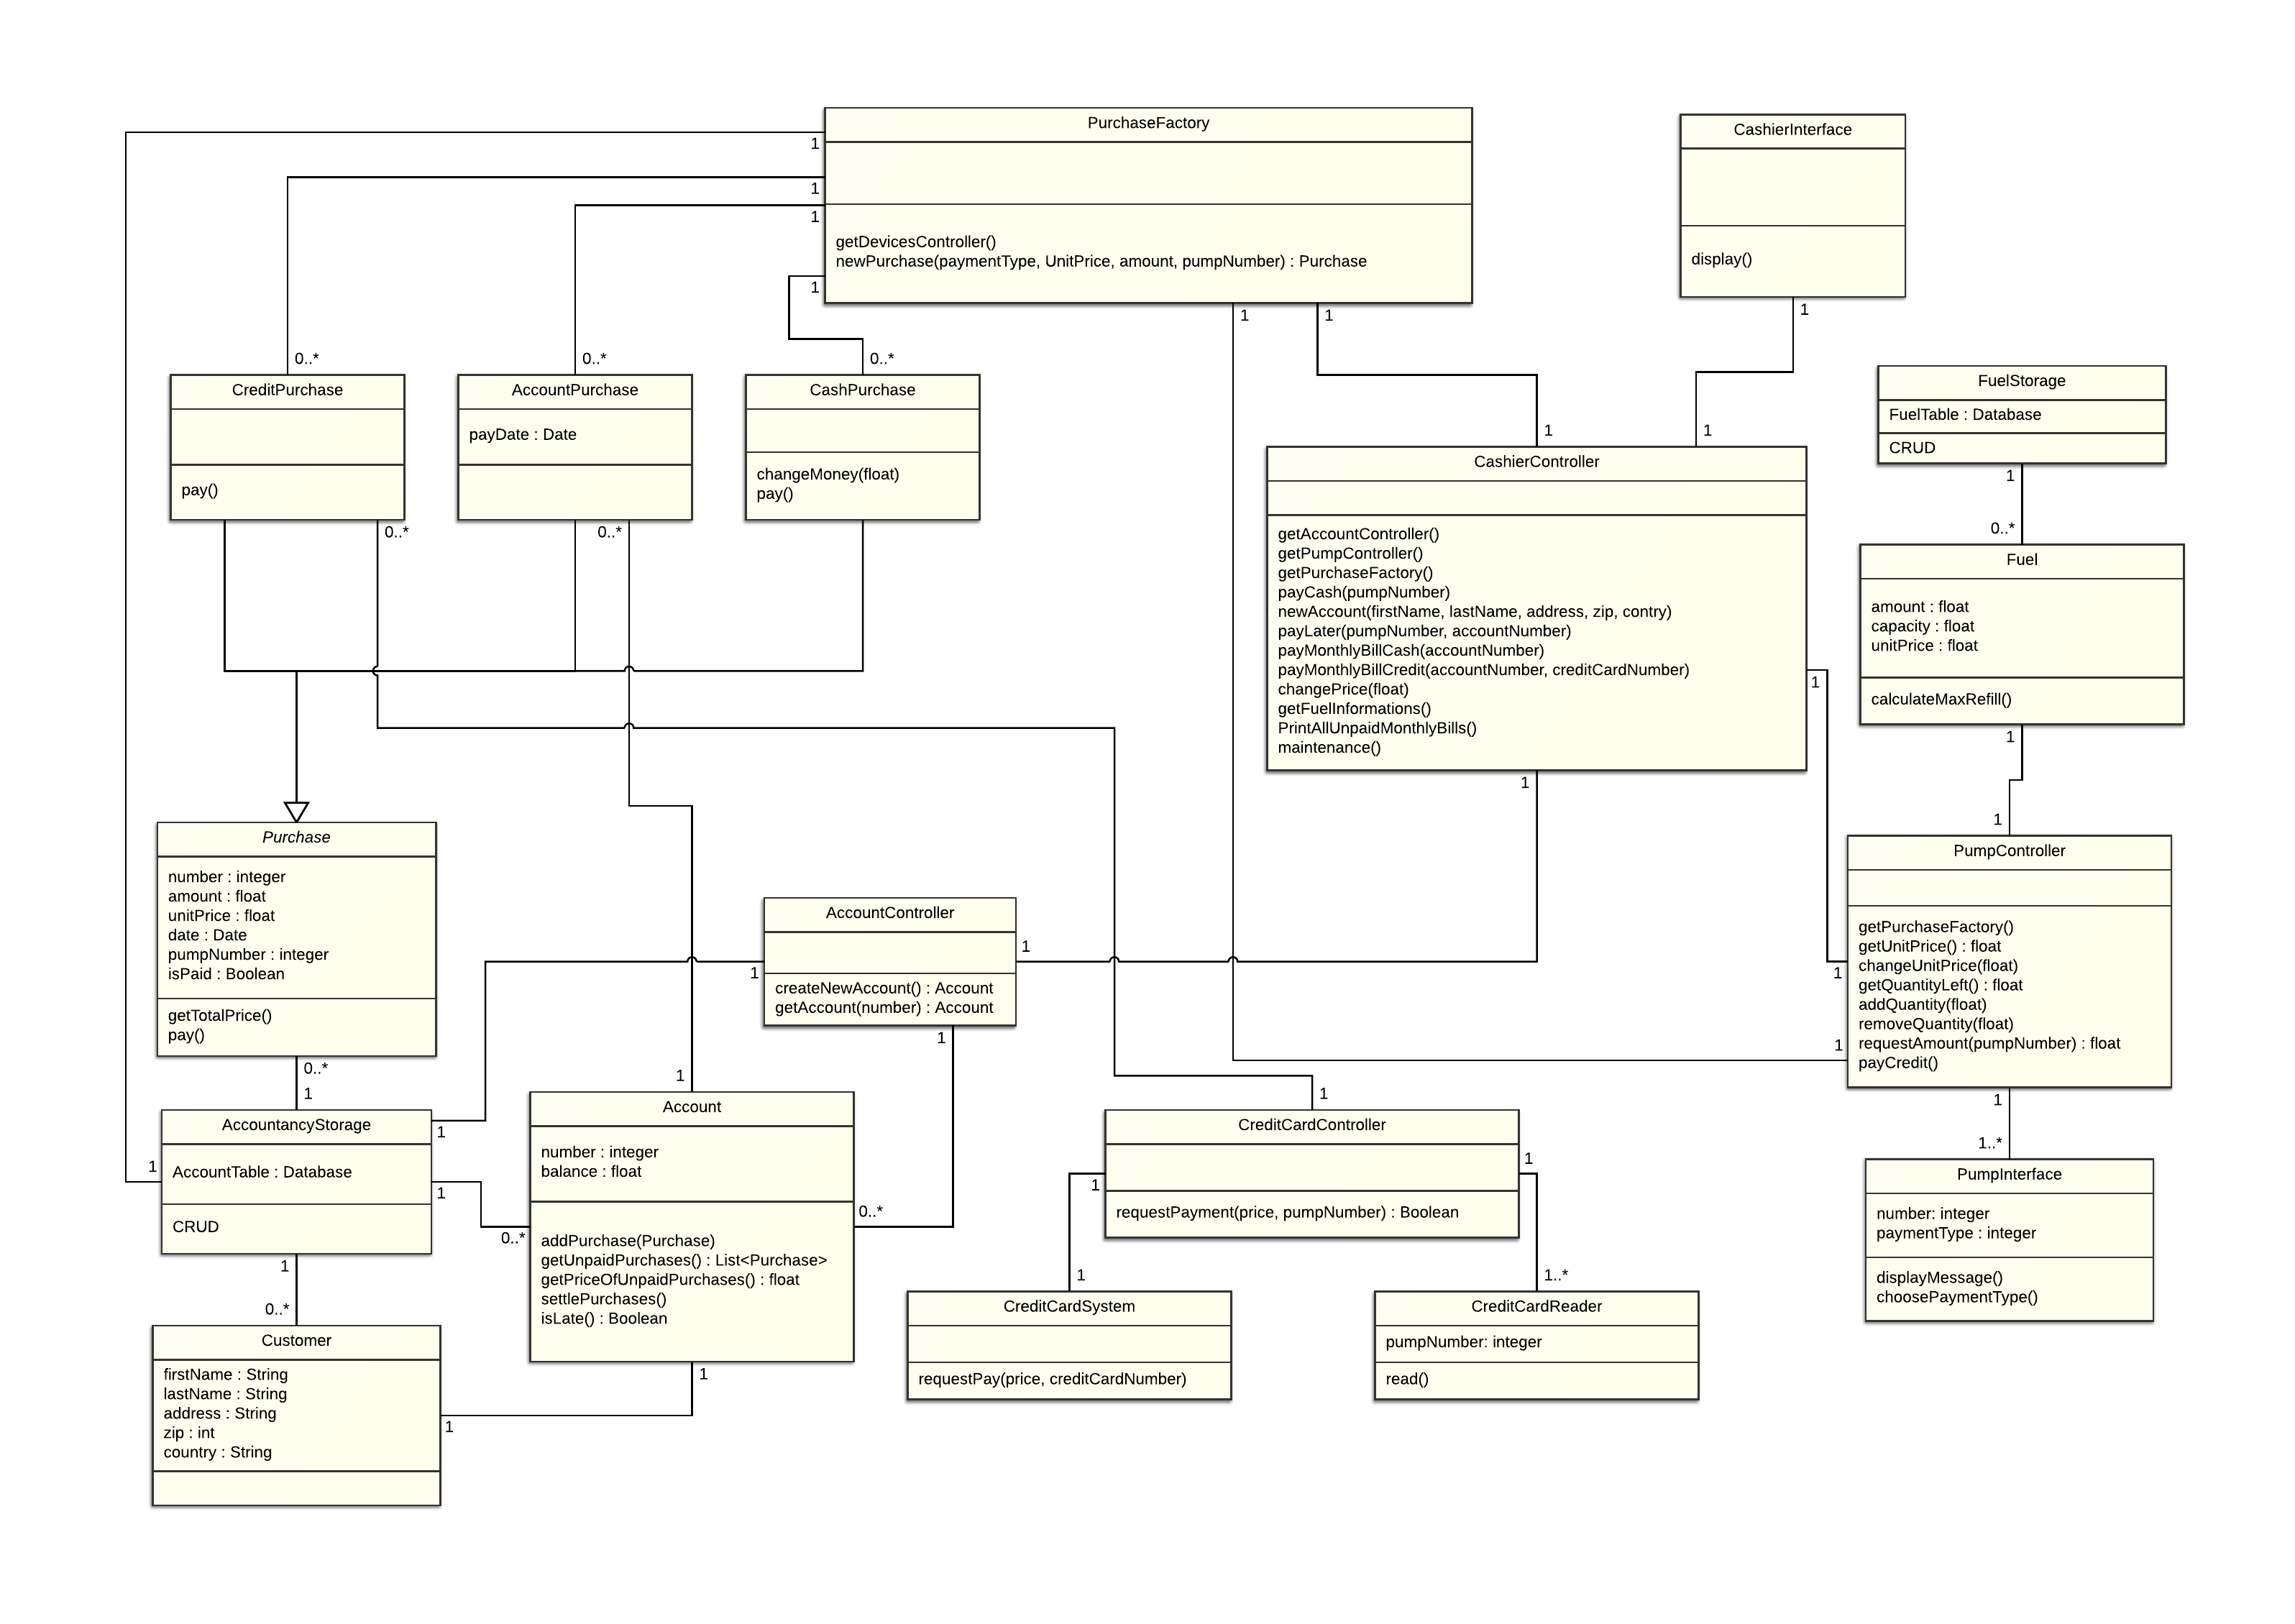
\includegraphics[angle=90, origin=c, width=1\textwidth]{uml.png}}
\end{center}

\subsection*{Short description}

\settextlisting

\subsubsection*{CashierController}
The \lstinline|CashierController| is the main controller. It is the entry point of the application. It will initialize the \lstinline|PumpController|, the \lstinline|AccountController|, the \lstinline|PurchaseController| and finally its interface (\lstinline|CashierInterface|).

\subsubsection*{CashierInterface}
This class is responsible of displaying the graphical user interface to the cashier.

\subsubsection*{PurchaseFactory}
The \lstinline|PurchaseController| is responsible of creating and saving new \lstinline|Purchase|.
If the purchase is a \lstinline|CreditPurchase|, the controller will interact with the \lstinline|CreditCardController| to directly settle the payment.

\subsubsection*{Purchase}
This abstract class represents a purchase.

\subsubsection*{CreditPurchase}
Specialized class for representing a purchase made via credit card.

\subsubsection*{AccountPurchase}
Specialized class for representing a purchase that is not directly paid. The purchase will be associated to a monthly bill account (\lstinline|Account| class).

\subsubsection*{CashPurchase}
Specialized class for representing a purchase made via cash.

\subsubsection*{Account}
This class is responsible for keeping up to date the accountancy of a customer.

\subsubsection*{AccountController}
This controller is responsible for creating new \lstinline|Account| and getting existing \lstinline|Account|.

\subsubsection*{Customer}
Class representing a customer.

\subsubsection*{AccountancyStorage}
\settextlisting
This class is responsible of the persistence (to keep in a database) of \mbox{classes :} \lstinline|Account|, \lstinline|Purchase| and \lstinline|Customer|. \\
It provides CRUD methods: \lstinline|create|, \lstinline|read|, \lstinline|update|, and \lstinline|destroy|.

\subsubsection*{CreditCardController}
This class will interact with the \lstinline|CreditCardReader| and the \lstinline|CreditCardSystem|.
It will offer a simple way to request a payment by manipulating the external APIs of the credit card company.
We need to know the \lstinline|pumpNumber| to enable the right card reader associated to a gas pump.

\subsubsection*{CreditCardSystem}
This class will wrap the external API of the credit card system.

\subsubsection*{CreditCardReader}
This class will wrap the external API of the credit card reader.

\subsubsection*{PumpInterface}
This class is responsible for displaying messages and listen to choices made by the user.

\subsubsection*{PumpController}
This controller manages everything related to the \lstinline|Fuel| stock. Since the user can pay directly by credit card at a pump, it can call the \lstinline|PurchaseFactory| to handle the payment.

\subsubsection*{Fuel}
Class for representing fuel stock.

\subsubsection*{FuelStorage}
This class is responsible of the persistence (to keep in a database) of the \lstinline|Fuel| stock.


\subsection*{USES diagram}

\begin{center}
\centerline{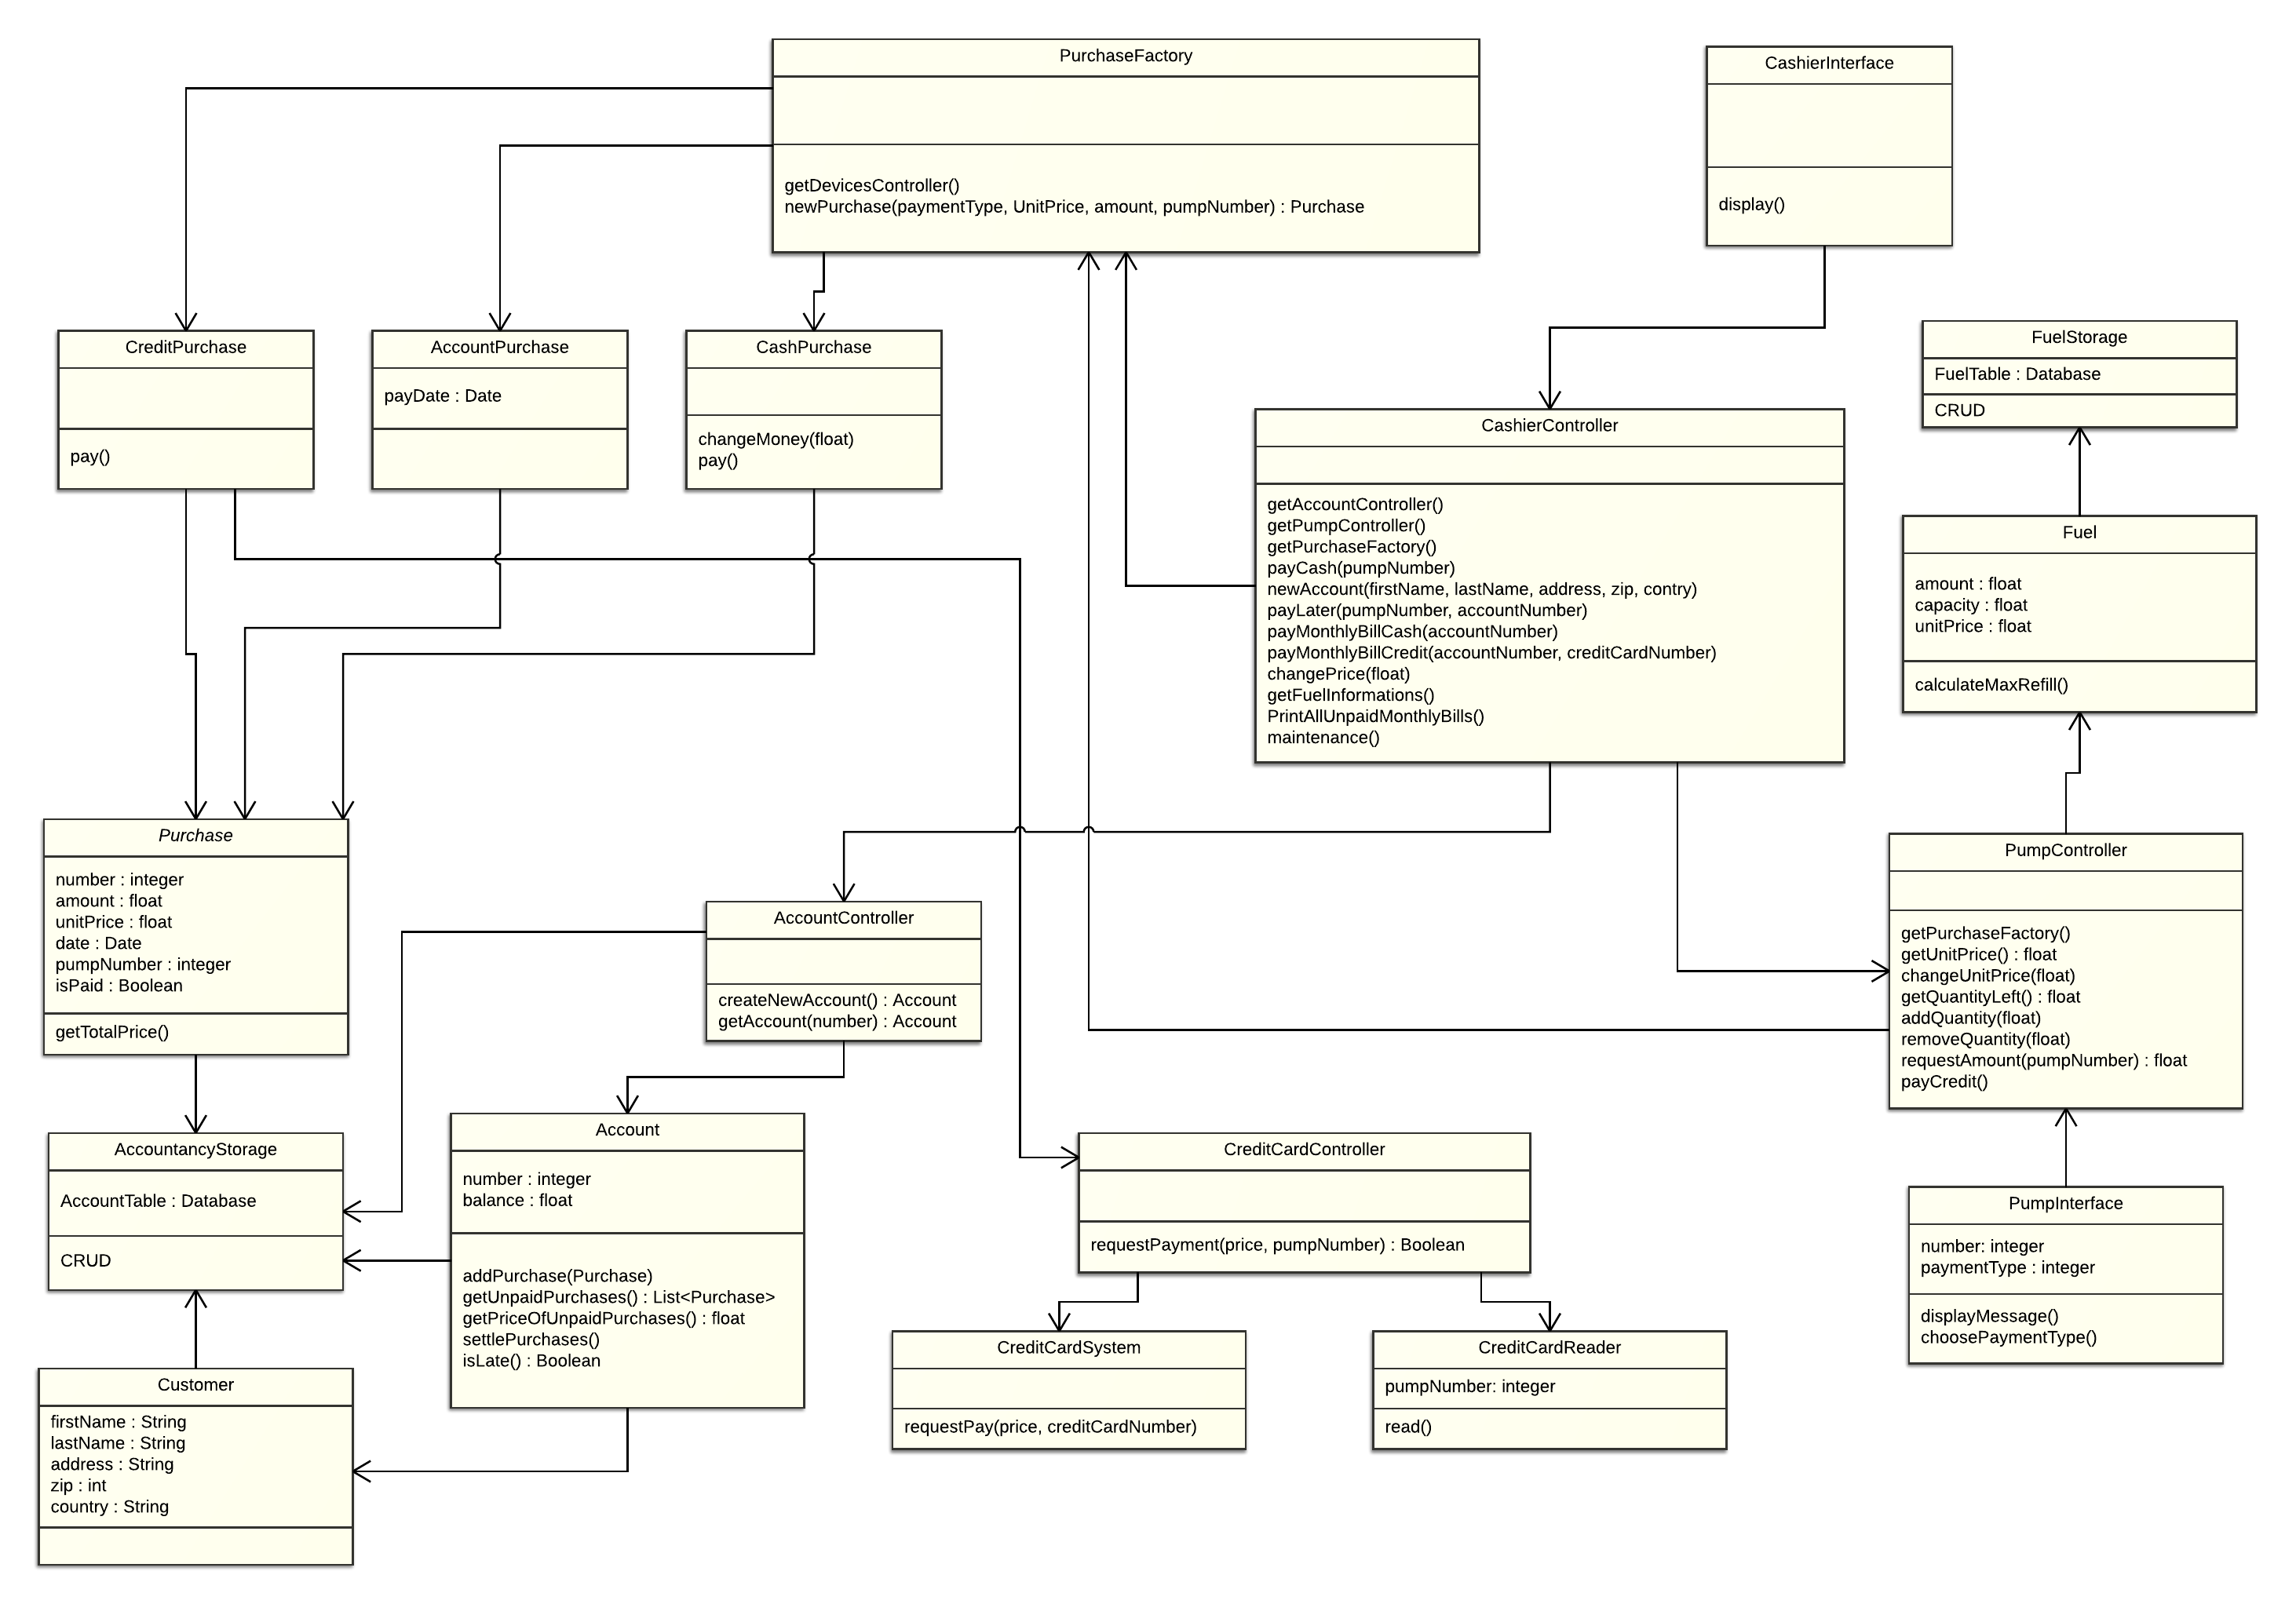
\includegraphics[angle=90, origin=c, width=1\textwidth]{use.png}}
\end{center}




\subsection*{Design Patterns}

\subsubsection{Template Method}

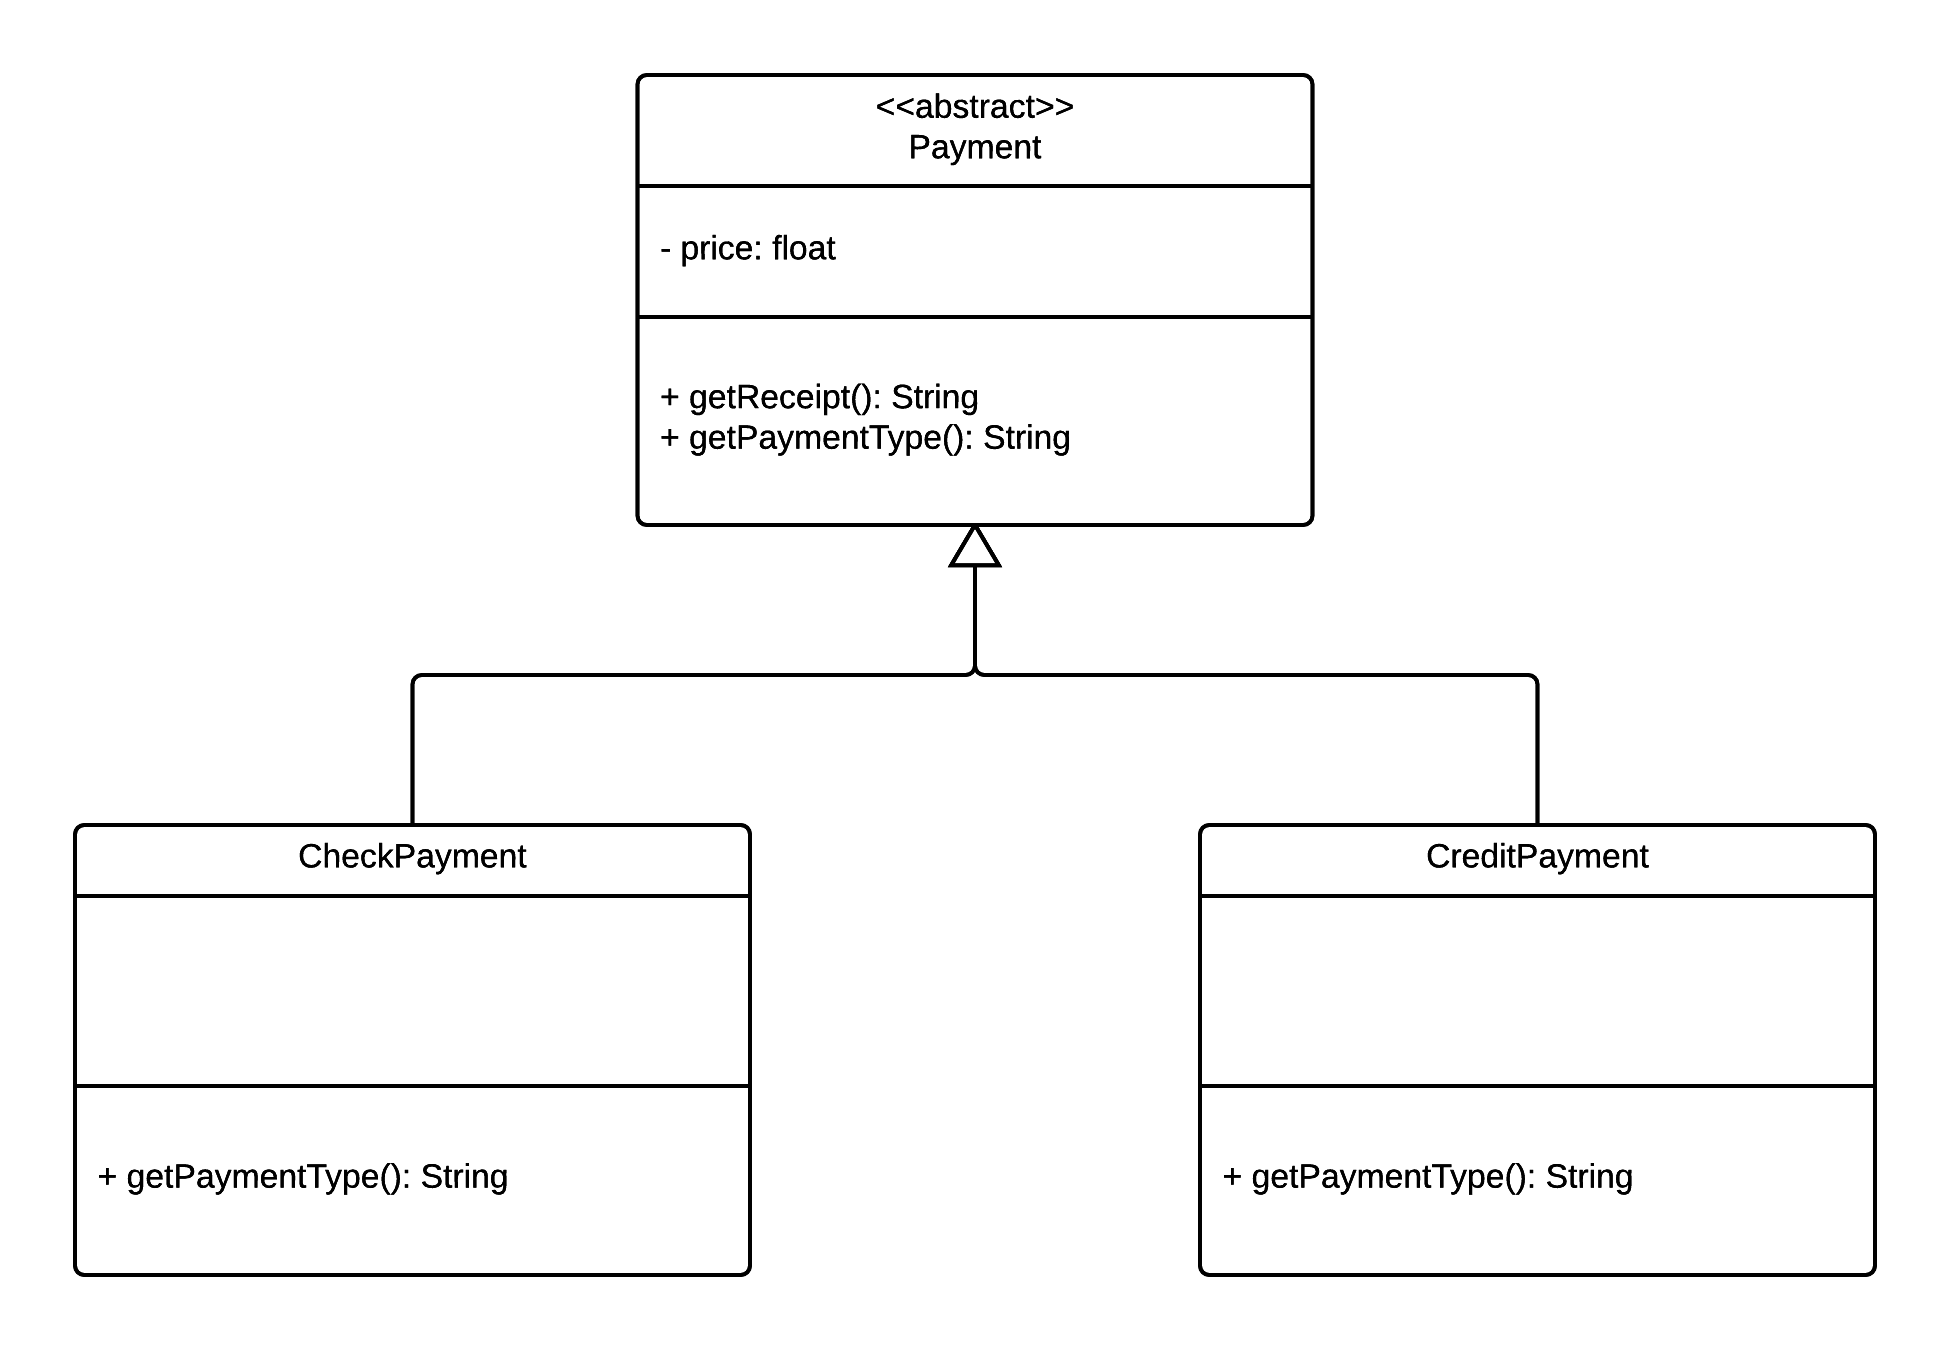
\includegraphics[width=\textwidth]{TemplateMethodPattern.png}

\medskip
\settextlisting
Any instance of \lstinline|Payment| has a method \lstinline|getReceipt()| that produces a printable receipt for the payment.
This method calls the \lstinline|getPaymentType()| method that subclasses of \lstinline|Payment| must implement.


\bigskip
\lstset{%
	basicstyle=\scriptsize\ttfamily,
}

\begin{lstlisting}
public abstract class Payment {
	public String getReceipt() {
		return "Payment by "+getPaymentType()+": "+this.price+"$";
	}
	
	public abstract String getPaymentType();
}
\end{lstlisting}


\begin{lstlisting}
class CheckPayment extends Payment {
	// ...
	private String getPaymentType() {
		return "check";
	}
	// ...
}
\end{lstlisting}


\begin{lstlisting}
class CreditPayment extends Payment {
	// ...
	private String getPaymentType() {
		return "credit card";
	}
	// ...
}
\end{lstlisting}




\subsubsection{Strategy pattern}

\centerline{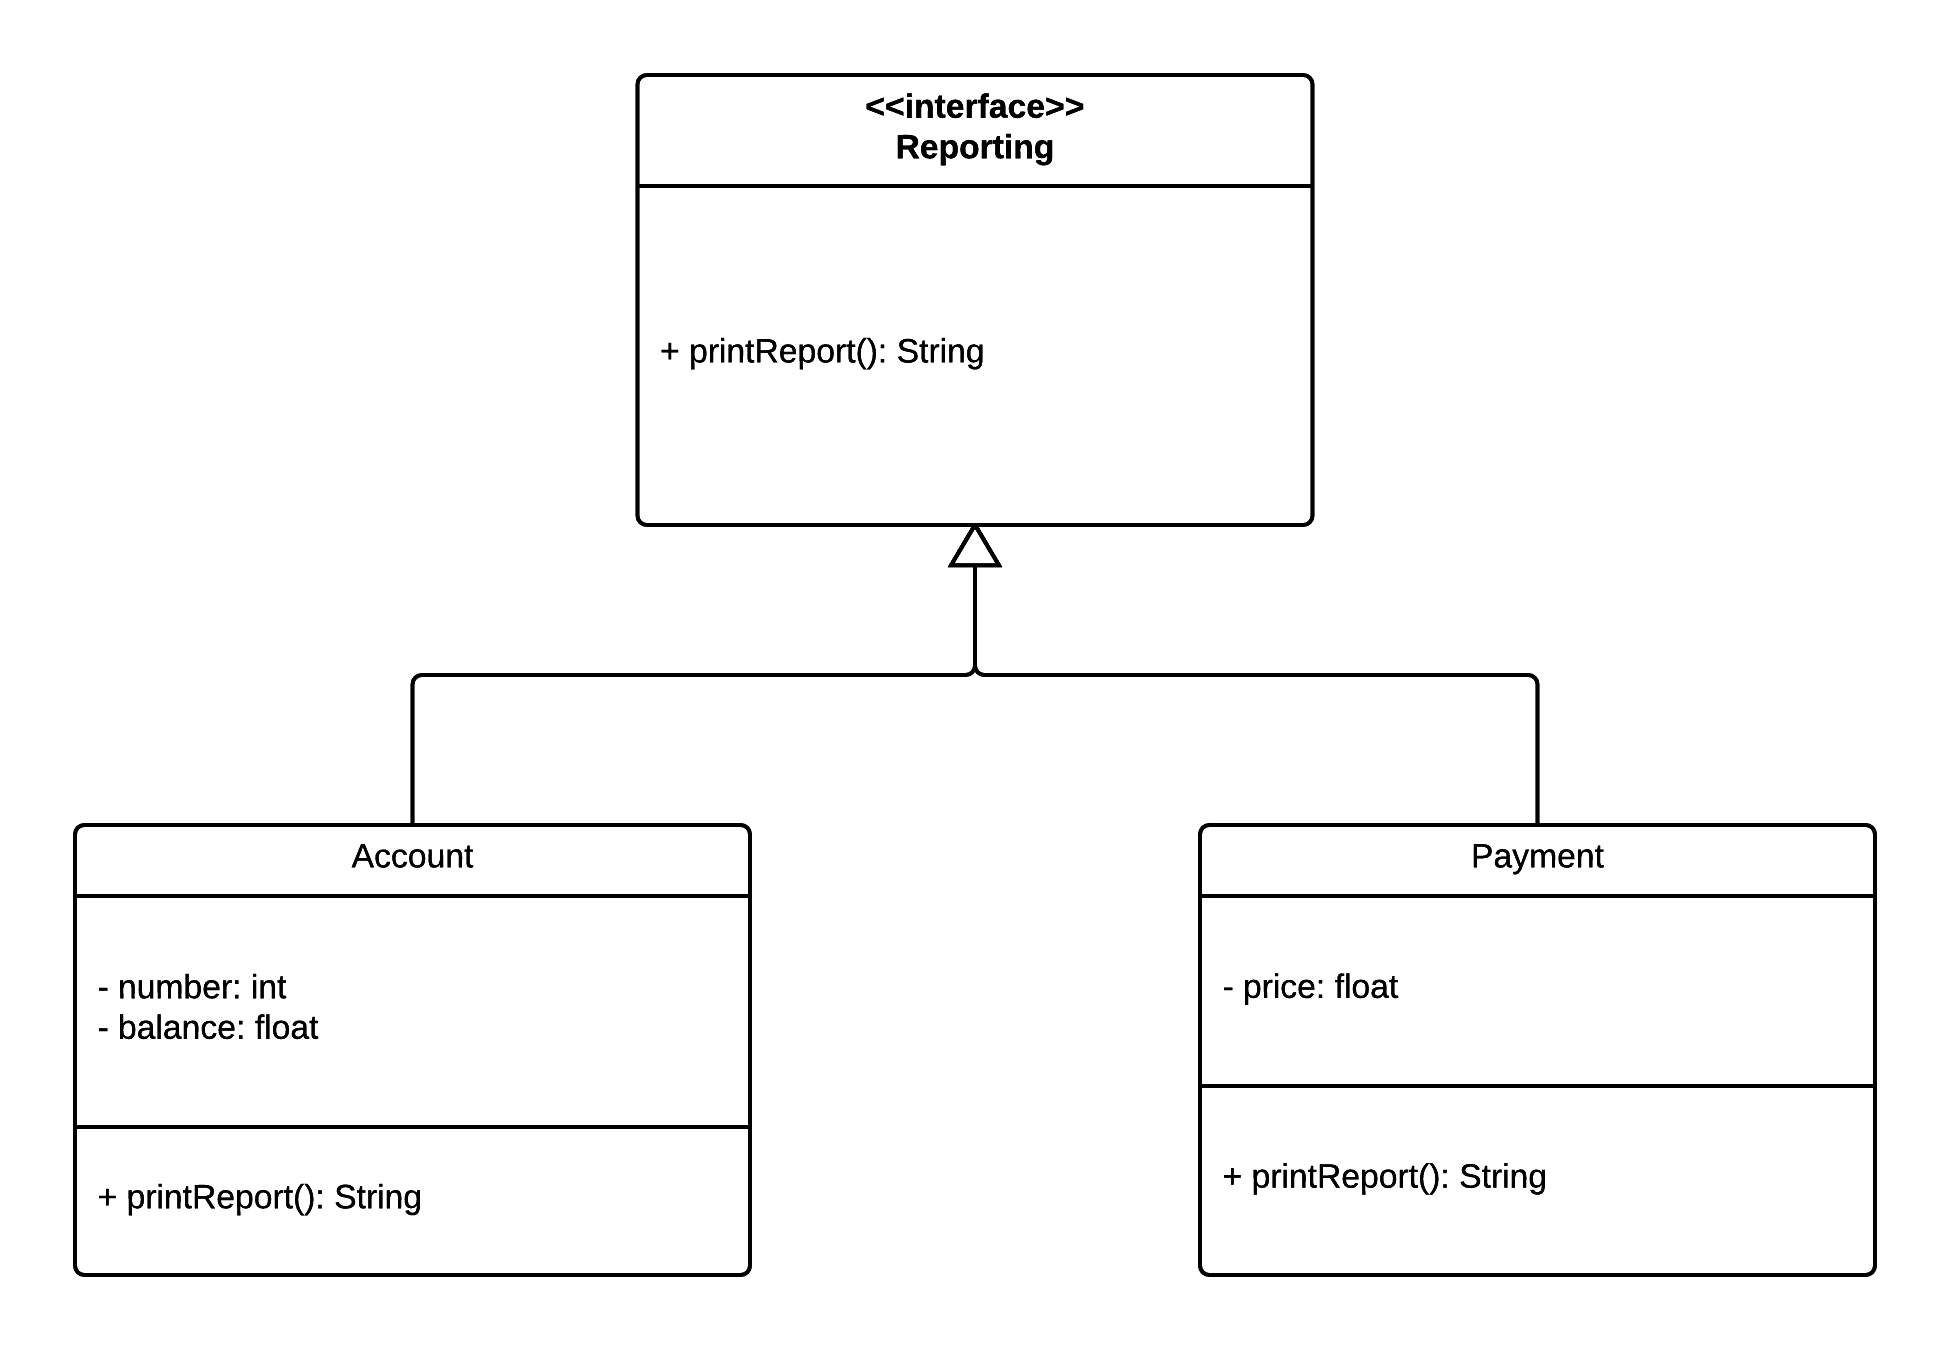
\includegraphics[width=0.9\textwidth]{StrategyPattern.png}}

\medskip
\settextlisting
The \lstinline|Reporting| interface advertises the \lstinline|printReport| method.
Each of the classes implementing \lstinline|Reporting| must define its own \lstinline|printReport| method.

\bigskip
%\setcodelisting
\lstset{ basicstyle=\scriptsize\ttfamily }
\begin{lstlisting}
public interface Reporting {
	public String printReport();
}
\end{lstlisting}


\begin{lstlisting}
public class Account implements Reporting {
	// ...
	public String printReport () {
		String report = "";
		List<Payment> payments = getPayments();
		for (Payment p : payments) {
			report += p.printReport()+"\n";
		}
		return report;
	}
	// ...
}
\end{lstlisting}


\begin{lstlisting}
public class Payment implements Reporting {
	// ...
	public String printReport () {
		String report = "Payment informations:\n"
					   +"Date: "+getDate()+"\n"
					   +"Amount: "+getTotalPrice()+"\n";
		return report;
	}
	// ...
}

\end{lstlisting}




\subsubsection{Decorator pattern}


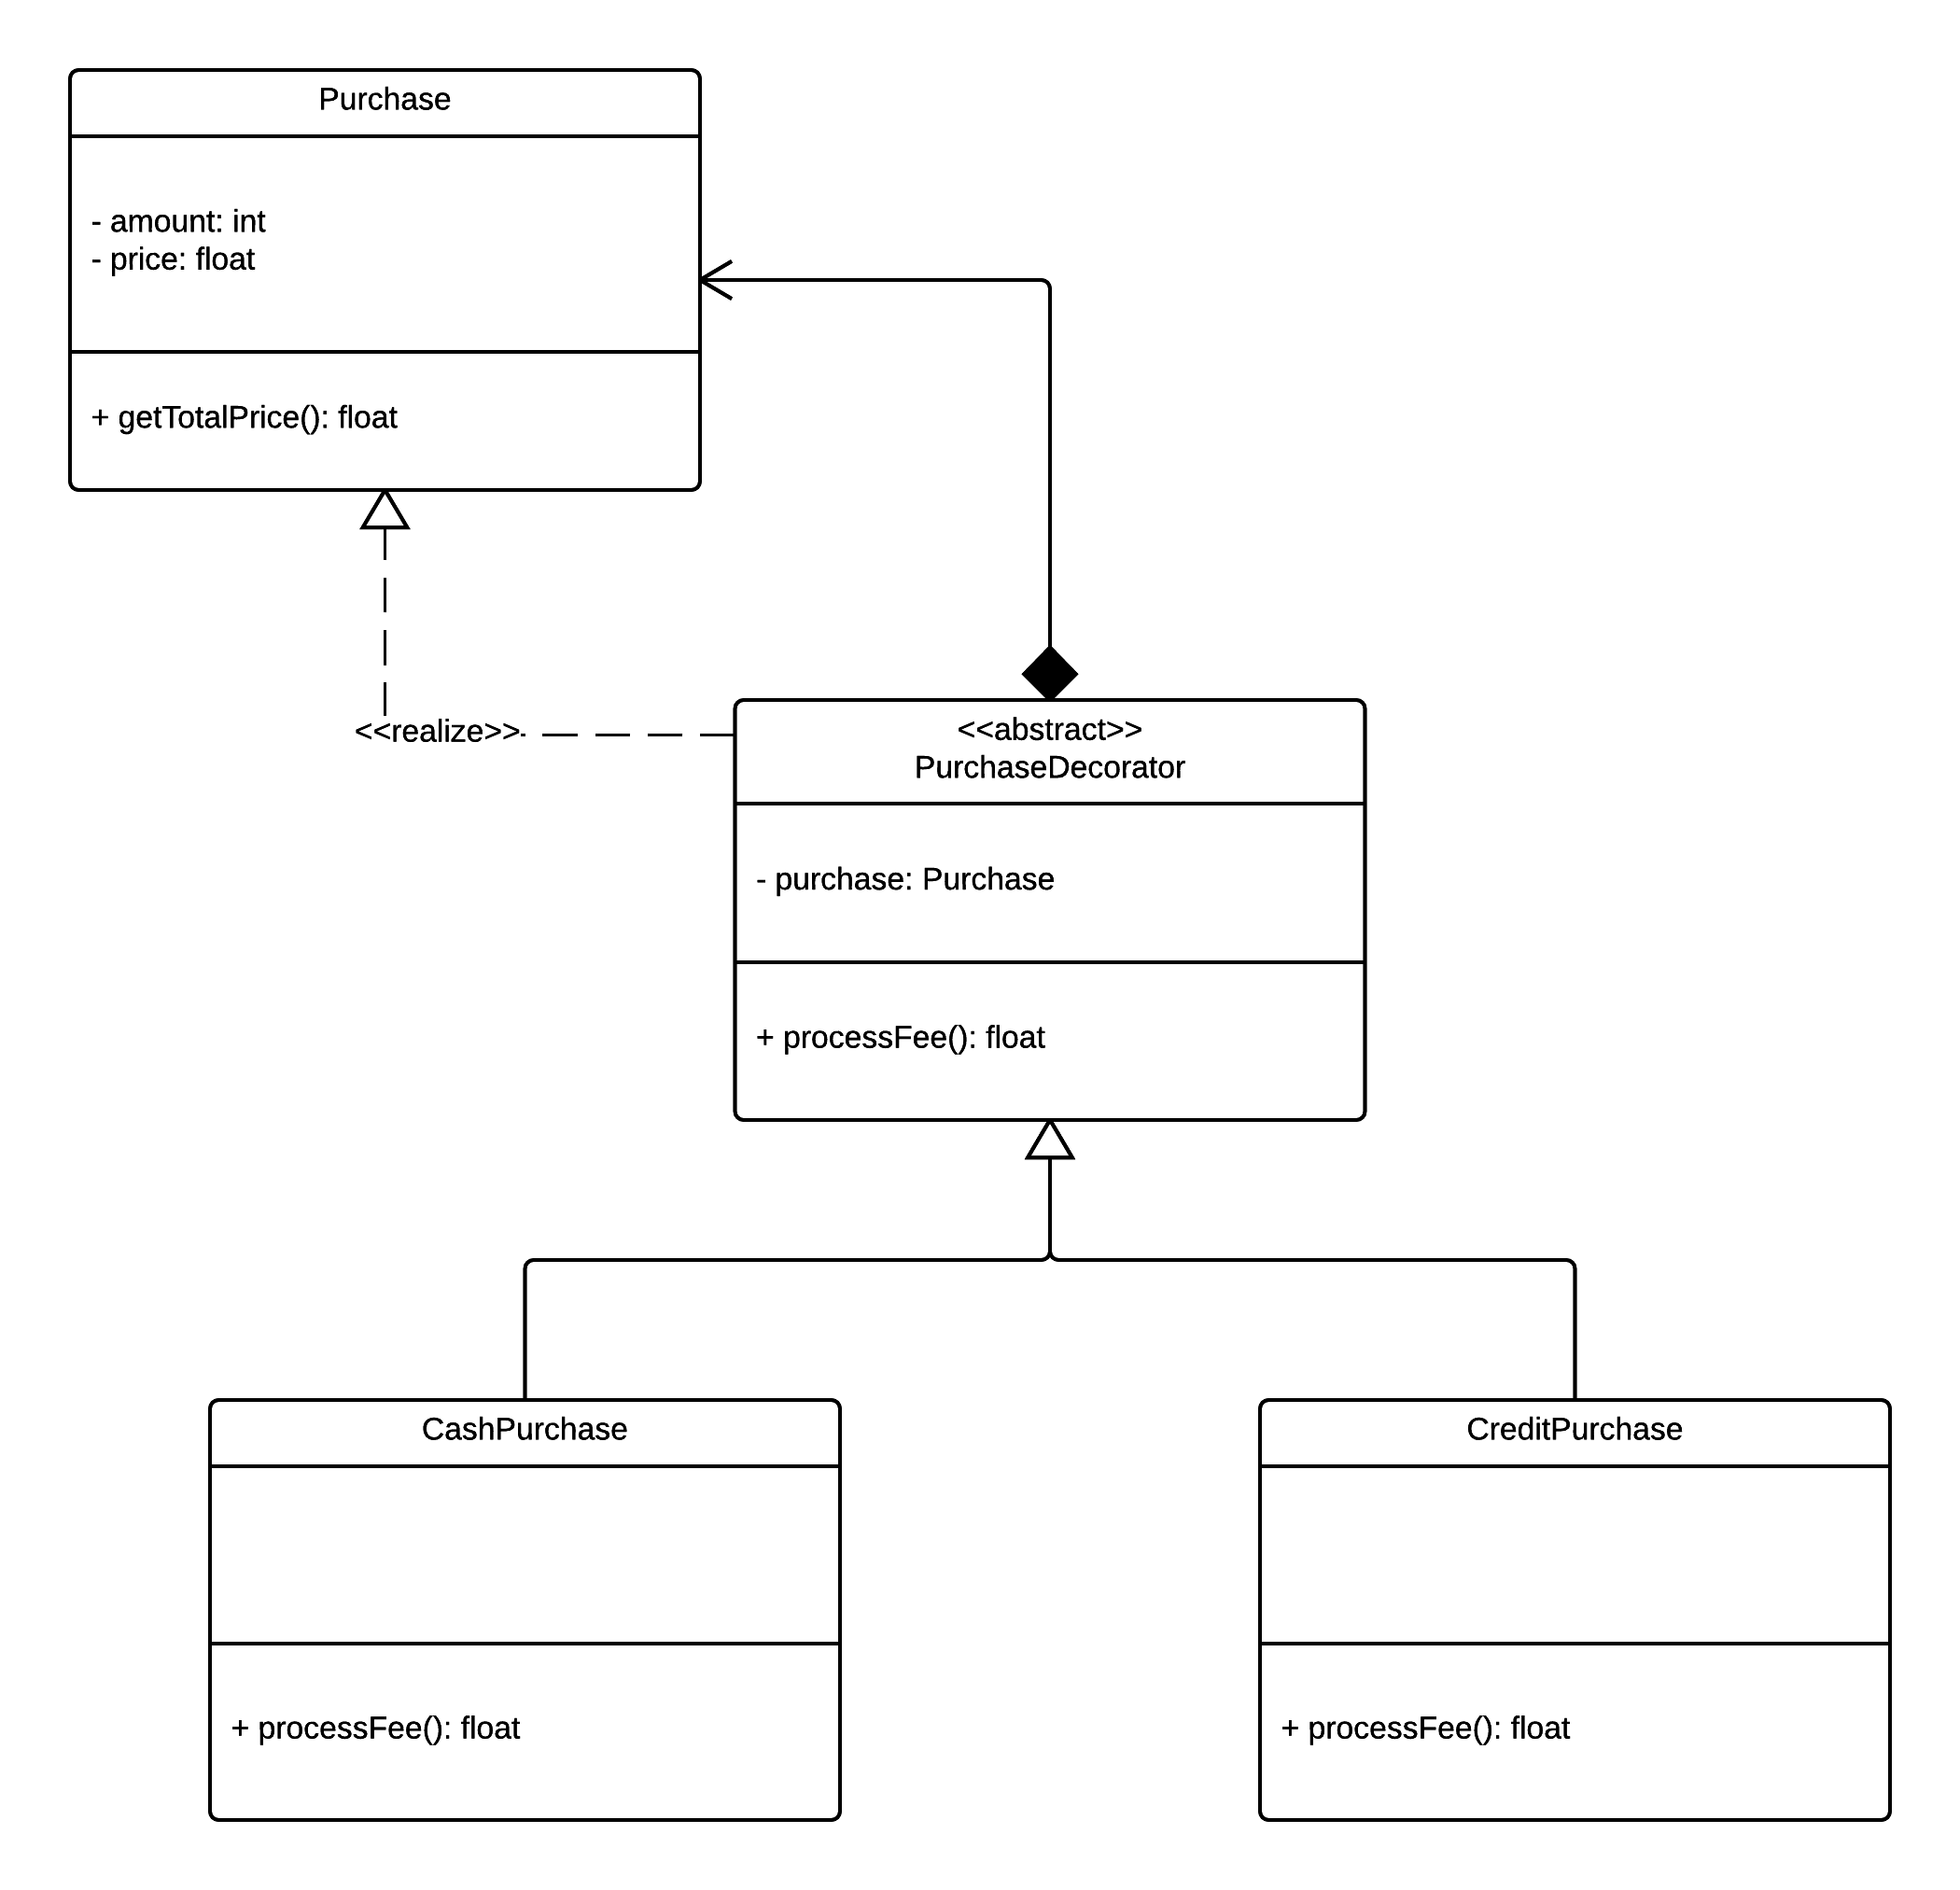
\includegraphics[width=\textwidth]{DecoratorPattern.png}

\medskip
\settextlisting
The \lstinline|PurchaseDecorator| class inherits from \lstinline|Purchase|, and contains a \lstinline|Purchase| object.
Classes that inherit from \lstinline|PurchaseDecorator| can add or remove functionalities at runtime.

\bigskip
\setcodelisting
\begin{lstlisting}
public class Purchase {
	// ...
}
\end{lstlisting}


\begin{lstlisting}
public abstract class PurchaseDecorator extends Purchase {
	protected Purchase purchase;
	
	public PurchaseDecorator (Purchase p) {
		this.purchase = p;
	}
	
	public abstract float processFee();
}
\end{lstlisting}


\begin{lstlisting}
public class CashPurchase extends PurchaseDecorator {
	// ...
	public float processFee() {
		return getTotalPrice() + 0.50;
	}
}
\end{lstlisting}


\begin{lstlisting}
public class CreditPurchase extends PurchaseDecorator {
	// ...
	public float processFee() {
		return getTotalPrice() * 1.05;
	}
}
\end{lstlisting}




\subsubsection{Observer Pattern}

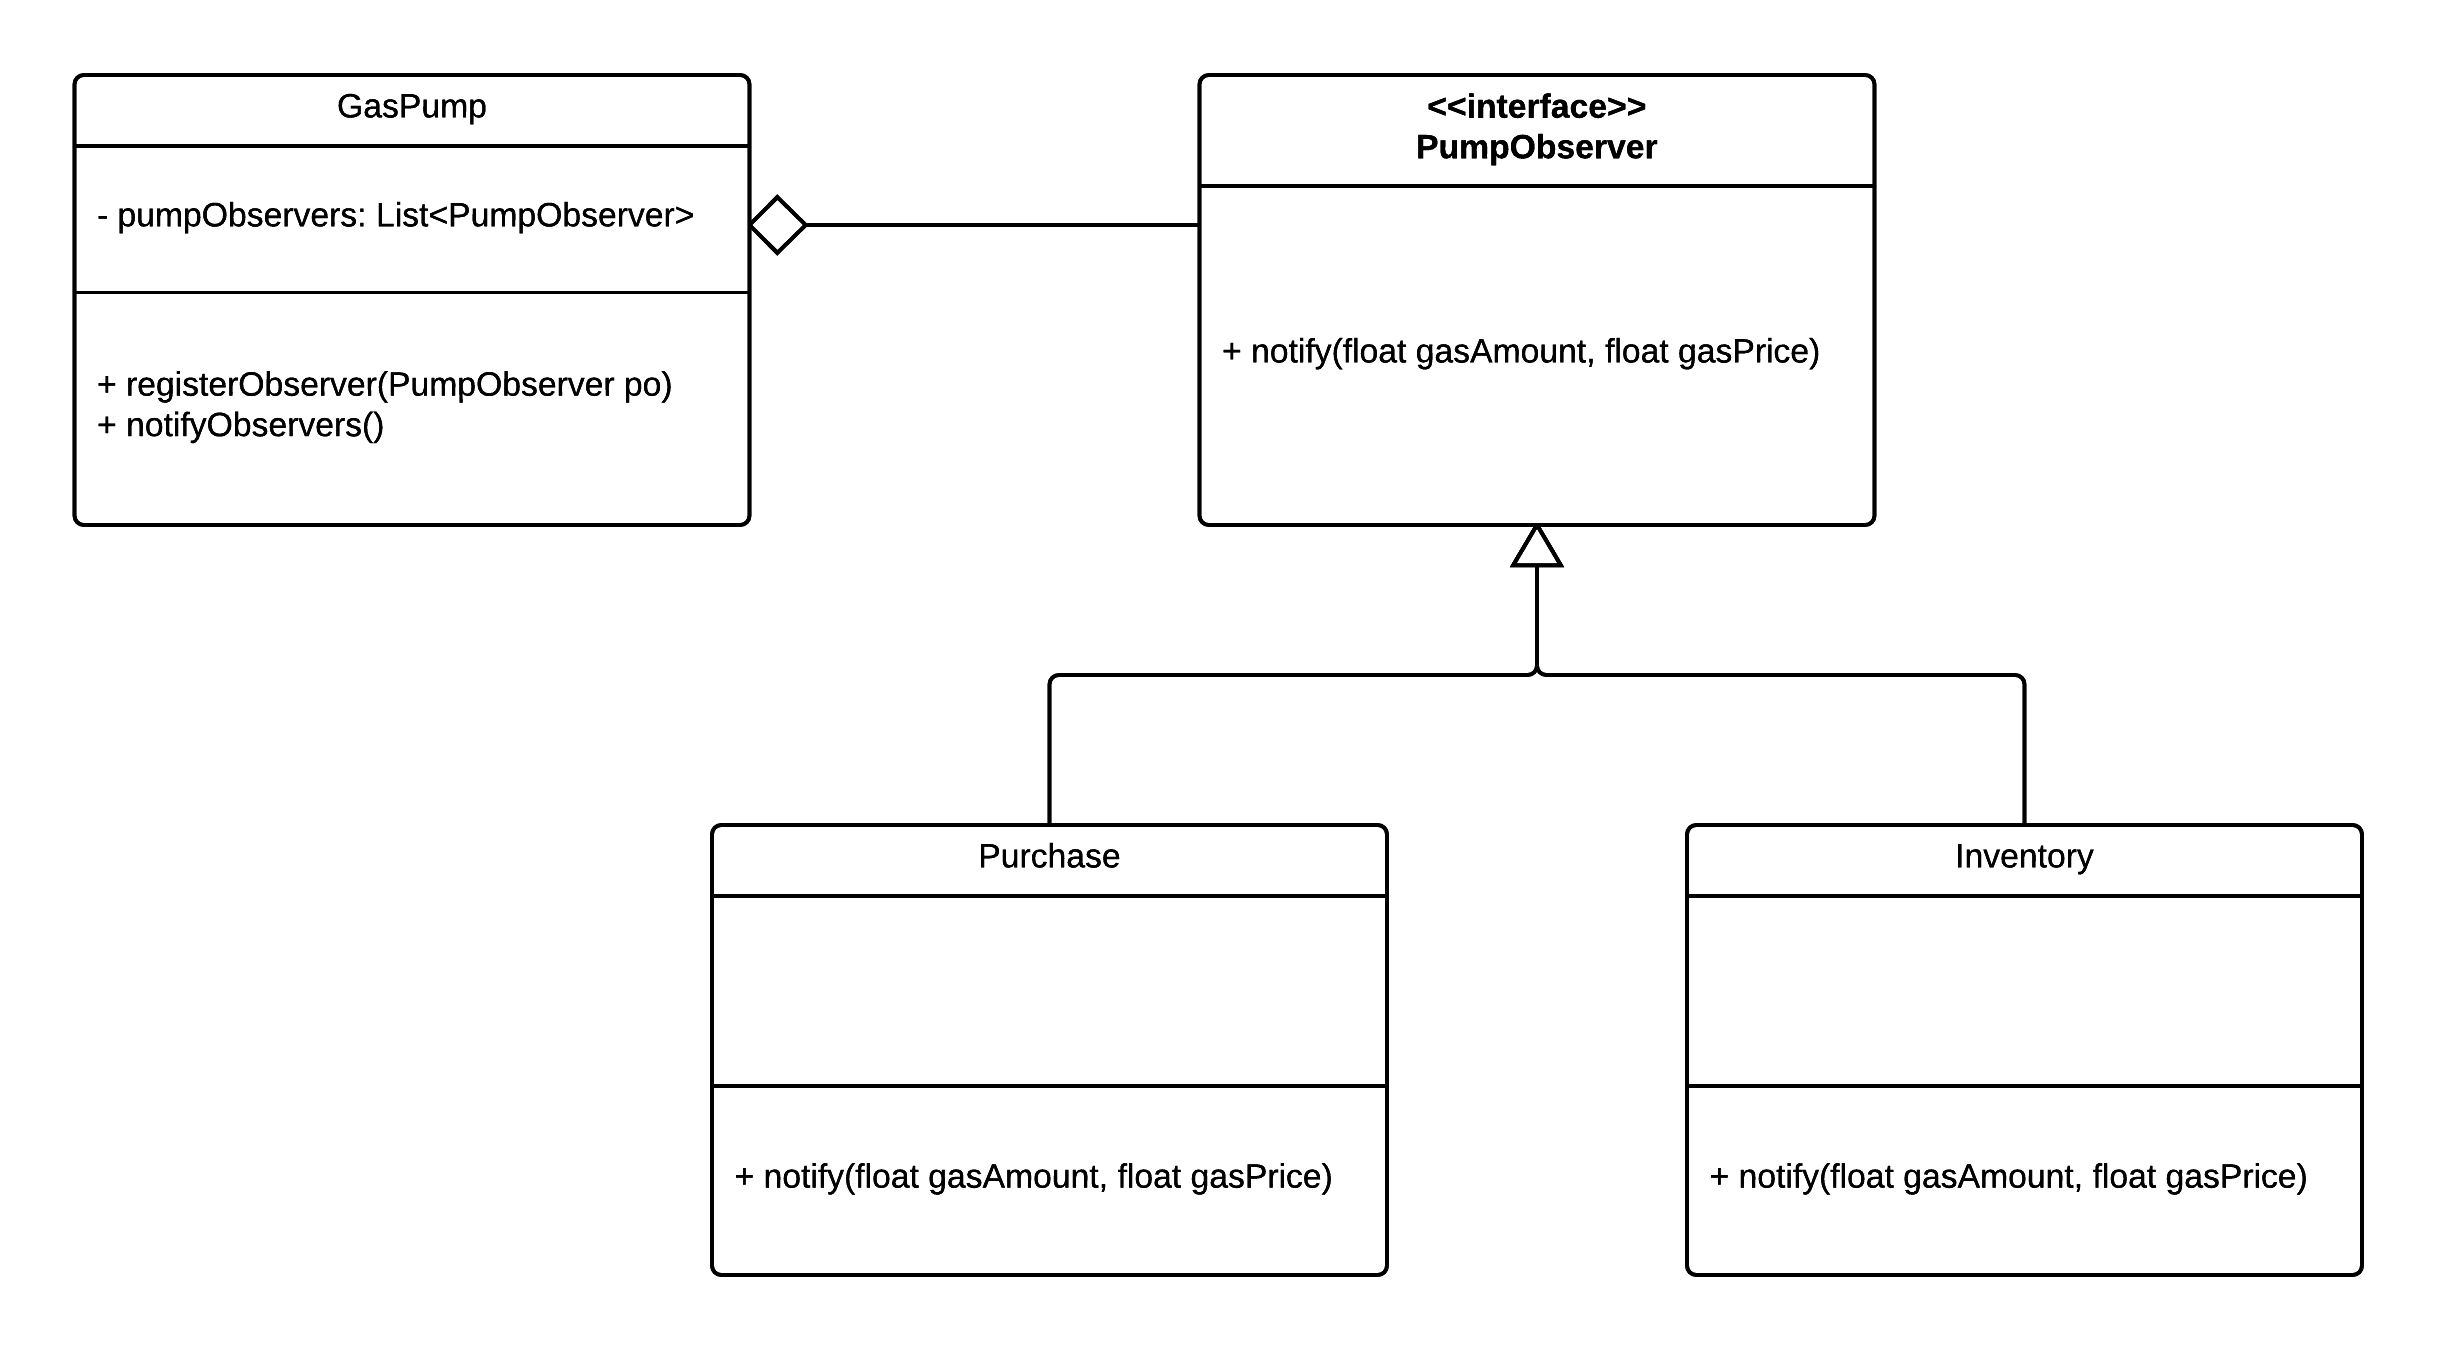
\includegraphics[width=\textwidth]{ObserverPattern.png}

\settextlisting
The \lstinline|GasPump| has a collection of \lstinline|PumpObserver|.
When the customer hangs up the nozzle, the \lstinline|GasPump| executes the \lstinline|notifyObservers| method, which is responsible for notifying to the observers the amount and the price of gas that the customer dispensed.

\bigskip
\setcodelisting
%\lstset{ basicstyle=\scriptsize\ttfamily }
\begin{lstlisting}
public class GasPump {
	private List<PumpObserver> pumpObservers;
	// ...
	public void registerObserver(PumpObserver po) {
		this.pumpObservers.add(po);
	}
	
	public void notifyObservers () {
		float dispensedGasAmount = getDispensedGasAmount();
		float dispensedGasPrice = getDispensedGasPrice();
		for (PumpObserver po : this.pumpObservers) {
			po.notify(dispensedGasAmount, dispensedGasPrice);
		}
	}
}
\end{lstlisting}


\begin{lstlisting}
public interface PumpObserver {
	public void notify(float gasAmount, float gasPrice);
}
\end{lstlisting}


\begin{lstlisting}
public class Purchase implements PumpObserver {
	// ...
	public void notify (float gasAmount, float gasPrice) {
		// ...
	}
}
\end{lstlisting}


\begin{lstlisting}
public class Inventory implements PumpObserver {
	// ...
	public void notify (float gasAmount, float gasPrice) {
		// ...
	}
}
\end{lstlisting}




\subsubsection{Composite Pattern}

\centerline{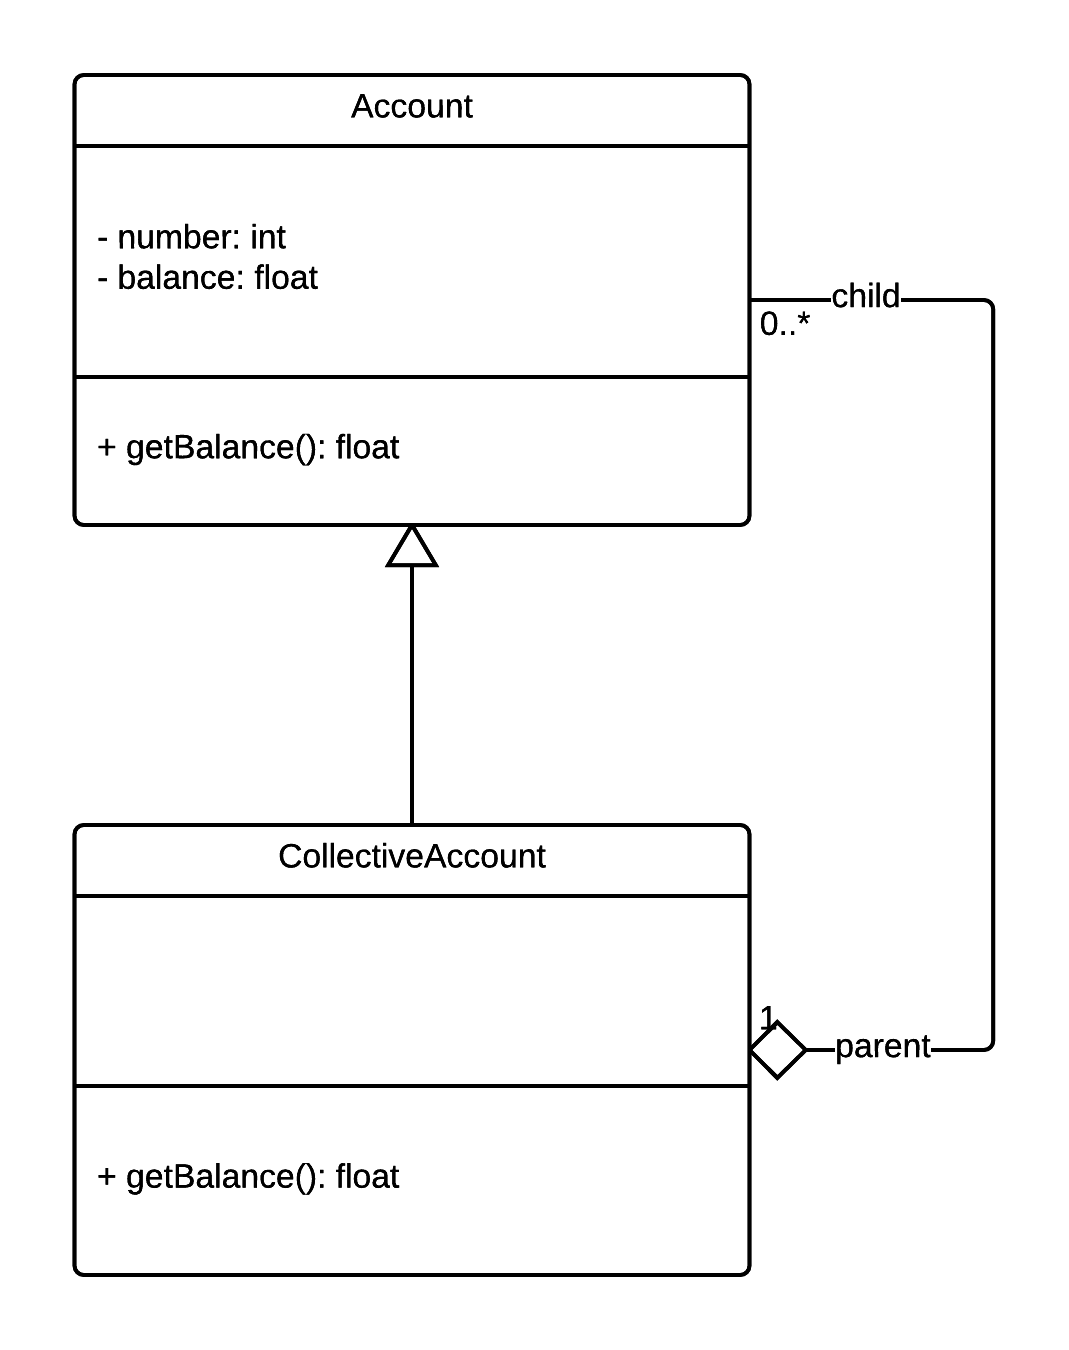
\includegraphics[height=9cm]{CompositePattern.png}}

\settextlisting
The \lstinline|CollectiveAccount| is at the same time an \lstinline|Account|, but also an aggregation of \lstinline|Account|s.
The composite pattern allows to treat composite and non-composite components uniformly.

\bigskip
\setcodelisting
\begin{lstlisting}
public class Account {
	protected int number;
	private float balance;
	
	public float getBalance() {
		return this.balance;
	}
}
\end{lstlisting}


\begin{lstlisting}
public class CollectiveAccount extends Account {
	List<Account> accounts;
	// ...
	
	public float getBalance() {
		float total = 0.0;
		for (Account a : accounts) {
			total += a.getBalance();
		}
		return total;
	}
}
\end{lstlisting}



\end{document}
